\begin{tikzpicture}[remember picture]
  \node (pic) at (0,0) {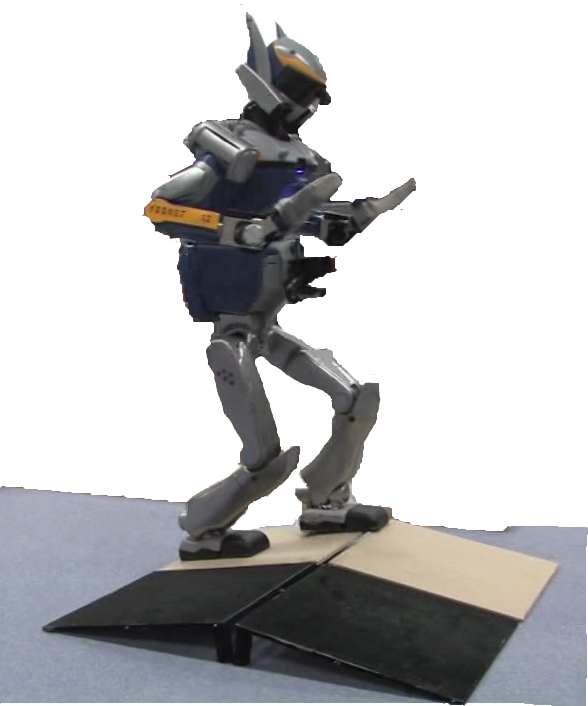
\includegraphics[width=0.38\paperwidth]{./images/HRP-2-Nishiwaki-Alone}};
%  \node (pic) at (2.7,3.6) {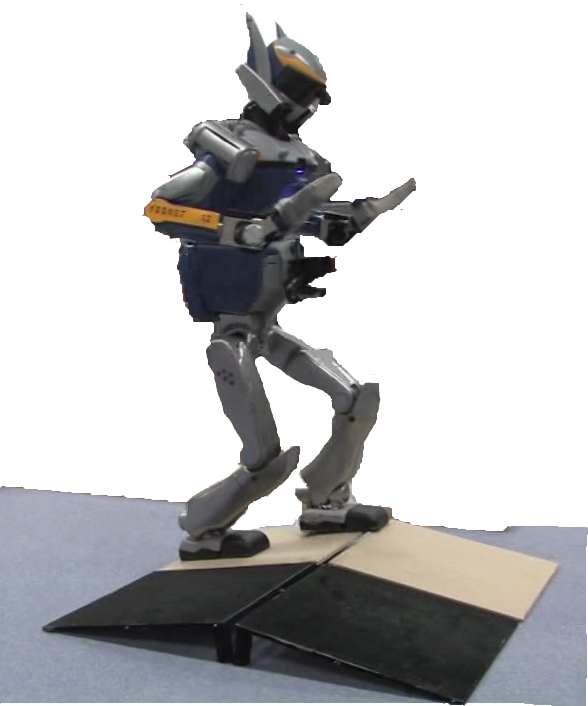
\includegraphics[width=0.8\linewidth]{./images/HRP-2-Nishiwaki-Alone}};

%  \draw[help lines] (1,1) grid (5,6);         
%  \draw (0,0) {(0,0)};         
  \node (com) at ([shift={(-0.2,0.8)}]pic) {};
  \draw[color=black,fill=white,line width=0.3mm,rotate around={40:(2.3,4.1)}] ([shift={(-0.2,0.2)}]com) ellipse (0.6cm and 0.4cm);
  \draw[color=black,fill=white,line width=0.3mm] (com) arc (0:360:0.3cm);
  \draw[fill=black] ([shift={(-0.3,0.3)}]com) arc (90:180:0.3cm) -- +(0.3cm,0cm) -- +(0.6cm,0cm) arc(360:270:0.3cm);
  
  \node (purparr) at ([shift={(-0.15,-0.1)}]com) {};
  \ExtractCoordinate{$(purparr)$};
  \draw[color=violet, left color=magenta, right color=magenta!60, 
    xshift=\XCoord,yshift=\YCoord, drop shadow={ashadow, color=magenta!60!black}] [rotate=180]
  \arrowtd;

  \node (lf) at ([shift={(-0.5,-1.63)}]pic) {};
  \ExtractCoordinate{$(lf)$};
  \draw[color=darkgreen, left color=green, right color=green!60, 
    xshift=\XCoord,yshift=\YCoord, drop shadow={ashadow, color=green!60!black}] [rotate=100,scale=0.15] 
  \arrowt;

  \node (rf) at ([shift={(0.4,-1.44)}]pic) {};
  \ExtractCoordinate{$(rf)$};
  \draw[color=darkgreen, left color=green, right color=green!60, 
    xshift=\XCoord,yshift=\YCoord, drop shadow={ashadow, color=green!60!black}] [rotate=100,scale=0.15] 
  \arrowt;
\end{tikzpicture}